\chapter{Revisión de la Literatura}
  \section{Redes Neuronales Artificiales}
  
    Las redes neuronales artificiales (RNA) son modelos computacionales de la Inteligencia Artificial los cuales contienen simples unidades de procesamientos llamadas neuronas.  Ellas se inspiran en el cerebro humano, tomando como base la conectividad entre neuronas y el aprendizaje que pueden tener.  Un perceptron o neurona (artificial) solamente resuelve problemas lineales y tiene la siguiente forma:
    
    \begin{figure}[H]
      \centering
      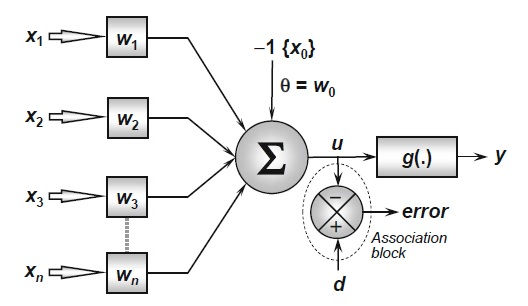
\includegraphics[width=\columnwidth]{ANN.jpg}
      \caption{Red Neuronal Artificial B\'asica}
      \label{fig:fig1}
    \end{figure}

    Donde $\Sigma$ es la representación matemática de la neurona.,  $x_1$, $x_2$,  \dots  ,$x_n$ son las variables de entrada a la red.  $w_1$,$w_2$,  \dots , $w_n$ son los pesos con los cuales se van a podnerar las entradas, es decir multiplicar cuando la información entra en la neurona. Posterior a multiplicar el peso por la entrada correspondiente,  se suman todos esos valores $w_1$$x_1$ + $w_2$$x_2$ + $w_3$$x_3$.

    Al revisar esta formula, se puede observar que se parece a la operación de una regresión la cual es:  $y$ = $w_0$ + $w_i$$x_i$,  de esta forma, internamente la neurona realiza una regresión lineal. En su contraparte, el parámetro que permite a la neurona trazar una recta cruzando el eje $y$ en el plano cartesiano (eje de las ordenadas), a ello se conoce como sesgo (del inglés $bias$),  este valor se agrega a la conexión, el cual usualmente se le da un valor de 1.
    Agregando este nuevo valor a la fórmula, queda de la siguiente manera: $ y = \Sigma w_i x_i + w_0 b$,  donde \textit{b} es el sesgo.

    Un inconveniente del uso de una sola neurona para experimentos es que solo va a resolver ejercicios parecidos a la puerta lógica AND u OR.
    
    Existen problemáticas de solo usar una sola neurona e.g problemas de tipo compuerta XOR.

    Para solucionarlo se usan dos o más neuronas, además de la función de activación, que es la que permite pasar la informaicón de una neurona a otra, en un rango especificado, y la cual se describirá en la siguiente sección.

    \subsection{Función de Activación}

      Dicho método se utiliza cuando el modelo de RNA contiene dos o más neuronas.
      Esta función lo que provoca es dar al modelo una salida no lineal, para eso la segunda fórmula presentada es distorcionada para quedar de la siguiente manera: $f( w_1x_1 + w_2x_2 + w_3x_3 + b_0)$ para el caso de 3 entradas.
      
      Al hablar de funciones de activación se deben de comentar las más comunes, como lo es la función escalonada.

      Tenemos la función escalonada, la cual se representa con la siguiente formula: 
      \[f(x) = \left\{ \begin{array}{lr} 0 & : x < 0\\ 1 & : x \ge 0 \end{array} \right. \]

      Su representación grafica queda de la siguiente manera:
      \begin{figure}[H]
        \centering
        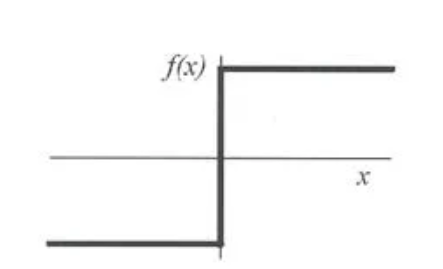
\includegraphics[width=5cm]{staggered.png}
        \caption{Función Escalonada}
        \label{fig:Función Escalonada}
      \end{figure}
  \section{Aprendizaje Incremental}
    Con el pasar de los años la tecnología a evolucionado, eso quiere decir que el Aprendizaje Automático se ha actualizado y que la cantidad de datos va aumentado con más frecuencia.
    
    Se puede verificar como \textit{"Una tarea de aprendizaje es incremental si los ejemplos de entrenamiento usados para resolverla están disponibles en horas extras, generalmente uno a la vez"} \cite{GiraudCarrier2000}, si los resultados no se necesitan de manera urgente, este tipo de trabajos serán resueltos por algoritmos de aprendizaje no incremental. 

    Una área donde esto es de mucha utilidad es la \textit{Rob\'otica} porque este necesita estar en constante entrenamiento \cite{GiraudCarrier2000}.

    Dicha forma de aprender fue inspirada en la forma en que el humano aprende y esta más rápida, fue por esto que fue adoptada por el aprendizaje m\'aquina.

    Con el paso del tiempo se ha convertido en un paradigma del aprendizaje automático, aquí el aprendizaje toma el lugar de nuevos ejemplos para juntarlos y conforme van aprendiendo estos toman el lugar de los ejemplos ya aprendidos \cite{liu2015}.

    \subsection{Algoritmos de Aprendizaje Incremental}
      El algoritmo de aprendizaje incremental puede definirse como aquel que cumple los siguientes criterios:  
      1) Ser capaz de aprender y actualizarse con cada nuevo dato etiquetado o no etiquetado. 
      2) Conservar los conocimientos adquiridos previamente.
      3) No debe requerir el acceso a los datos originales. 
      4) Generar una nueva clase o cluster cuando sea necesario. Dividir o fusionar los clusters cuando sea necesario. 
      5). Ser de naturaleza dinámica con el entorno cambiante \cite{Deshmukh2013}.

      \begin{figure}[H]
        	\centering
        	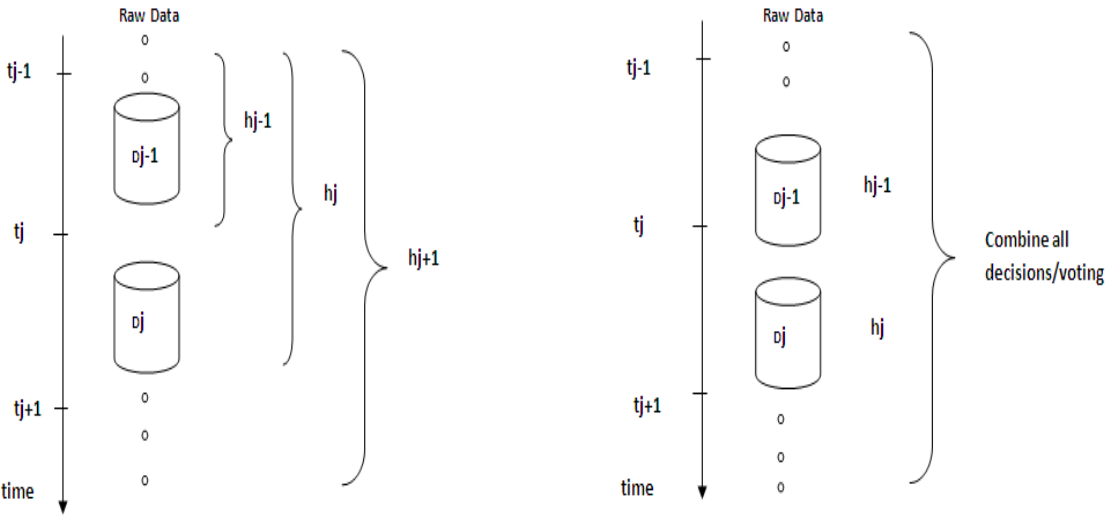
\includegraphics[width=\columnwidth]{MetodosAprendizajeIncremental.png}
            \caption{Dos enfoques tradicionales del aprendizaje incremental.}
            \label{fig:fig11}
        \end{figure} 
        1 Metodología de acumulación de datos. 2 Metodología de aprendizaje por conjuntos.\\
        
		Como se observa en la Figura 11, en el primer método, cuando se recibe una nueva porción de datos Dj, se descarta hj-1 y se desarrolla una nueva hipótesis hj, basada en todos los datos disponibles acumulados hasta el momento. 
		Y en el segundo método, cuando se recibe una nueva porción de datos Dj, se desarrolla una única hipótesis nueva o un conjunto de hipótesis nuevas basadas en los nuevos datos. 
		Por último, se puede utilizar un mecanismo de votación para combinar todas las decisiones de las diferentes hipótesis y obtener la predicción final.\\
		
		Por ejemplo, si se deja que Dj-1 represente la porción de datos recibida entre el tiempo tj-1 y tj, y que la hipótesis hj-1 se desarrolle sobre Dj-1.\\
		El sistema aprenderá información de forma adaptativa cuando se reciba una nueva porción de datos Dj.	
		En el método de aprendizaje por conjuntos, se desarrolla una nueva hipótesis hj o un conjunto de hipótesis H:h1, i1,2,...,M, basadas en los nuevos datos.  
		A continuación, se utiliza el mecanismo de votación para combinar todas las decisiones de las diferentes hipótesis y llegar a la predicción final.
		La mayor ventaja de este enfoque es que no se requiere almacenar los datos vistos anteriormente, el conocimiento se ha almacenado en la serie de hipótesis desarrolladas a lo largo de la vida de aprendizaje.\\
		
			Conocimiento en el momento t: \\
			Dt es un trozo de datos con n instancias (i=1,...,n) \\
			(xi,yi) es una instancia en el espacio de características m-dimensional X\\ 
			Yi $\in$ Y ={1,...,K} clases \\
			Función de distribución Df \\
			Una hipótesis ht, desarrollada por los datos basados en Dt con Pt \\
			La nueva entrada estará disponible en el momento (t+1) \\\\
			
			Algoritmo de aprendizaje:\\
			\begin{enumerate}
				\item Encontrar la relación entre Dt y Dt+1
				\item Actualizar la función de distribución inicial Dt+1
				\item Aplicar la hipótesis ht a Dt+1 y calcular el pseudoerror de ht
				\item Refinar la función de distribución para Dt+1
				\item Se desarrolla una hipótesis por los datos basados en Dt+1 con Pt+1
				\item Repetir el procedimiento cuando se reciba la siguiente porción del nuevo conjunto de datos.
			\end{enumerate}
			Resultado: La hipótesis final.\\